\section{Middleboxes: Design \& Implementation}
\label{sec:mbs}

In Table~\ref{tbl:mbreqs}, we introduced the set of middleboxes typically supported by outsourcing approaches and divided them in to Header, HTTP, and DPI middleboxes. 
We now revisit these middleboxes individually and discuss how they operate over the encrypted data.

\eat{
\begin{figure}[t]
  \centering
  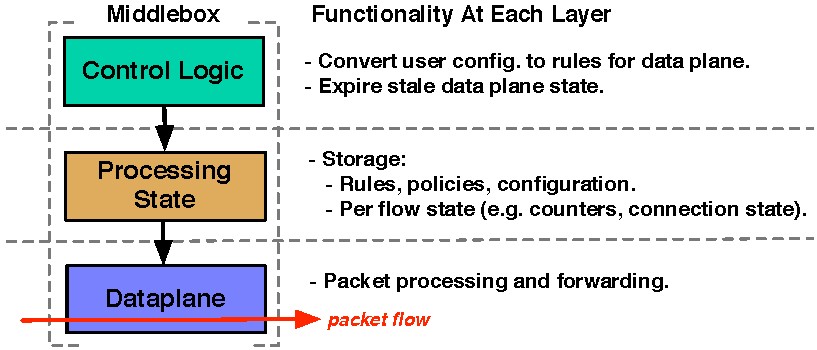
\includegraphics[width=3in]{fig/mbarch}
  \caption[]{\label{fig:mbarch} Typical middlebox software components. For most middleboxes, packet processing operations in the dataplane remain unmodified by \sys. \justine{Cut? Unnecessary?}}
\end{figure}
}

\subsection{Header Middleboxes}
Middleboxes which operate on IP and transport headers only include firewalls, NATs, and L4 load balancers.
Firewalls are read-only, but NATs and L4 load balancers may rewrite IP addresses or port values. 
For header middleboxes, per-packet operations remain unchanged for both read and write operations.

For read operations, the firewall receives a set of encrypted rueles from the gateway and compares them directly against the encrypted packets just as normal traffic.

For write operations, the middleboxes assign values from an address pool; it receives these encrypted pool values from the gateway during the rule generation phase.
These encrypted rules are marked with a special suffix reserved for rewritten values.
When the gateway receives a packet with such a rewritten value, it restores the plaintext value from the pool rather than decrypting the value from the options header for decryption.

\subsection{DPI Middleboxes}
We modify middleboxes which perform DPI operations as described by BlindBox~\cite{blindbox}.
The middleboxes search through the encrypted extension channel and block the connection if a blacklisted term is observed.

We modify DPI middleboxes relative to BlindBox as follows:



\subsection{HTTP Middleboxes}

\subsection{Implementation}

